Within T4.1 IIT developed in the first and the second year of the 
project a theoretical framework for estimating whole-body
dynamics from distributed multimodal sensors \cite{nori2015}. The sensors considered
include joint encoders, gyroscopes, accelerometers and force/torque sensors. In the third year of the project, IIT investigated the integration of this estimation techniques with the classical identification techniques for inertial parameters \cite{traversaro2015parametersEM}. For the fourth year the improvement of the reliability of the sensors was considered. More specifically the six axis force/torque sensors where discovered to have a change in behaviour after they are mounted on the robot. To tackle this an in-situ calibration procedure was developed.

The procedure used to calibrate the sensors in-situ takes advantage of the knowledge of the model of the robot to generate the expected wrenches of the sensors during some arbitrary motions. The wrenches used as reference are estimated through the model and kinematic measurements. It then uses this information to train and validate new calibration matrices, taking into account the calibration matrix obtained with a classical Workbench calibration.  This procedure was validated  on the F/T sensors mounted on the iCub humanoid robot legs and published in Humanoids 2016 \cite{Andrade}.


\begin{figure}
        \centering
        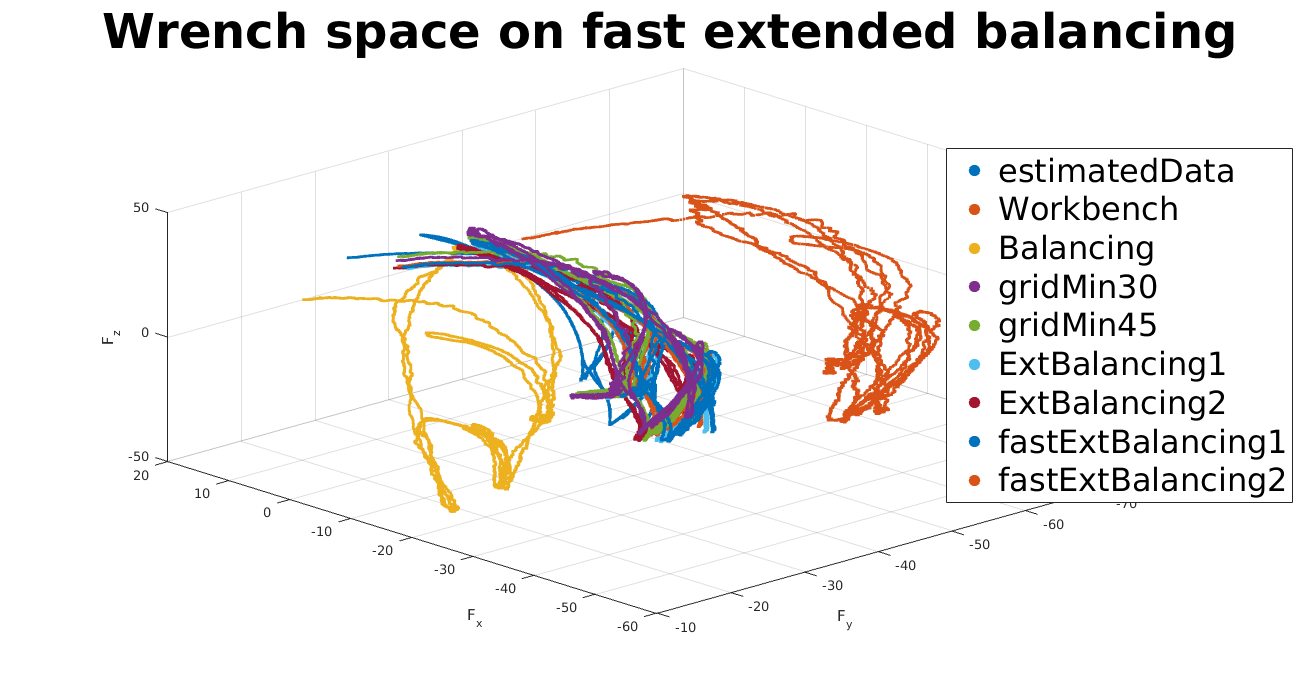
\includegraphics[width=\textwidth]{images/all1valid2.png}
        \caption{3D force comparison among the calibration matrices trained on each dataset against the model estimated forces on the fastExtBal1 dataset. }
        \label{fig:all1valid}
\end{figure}



% bibliography 
%@inproceedings{nori2015,
%  title={Simultaneous state and dynamics estimation in articulated structures},
%  author={Nori, Francesco and Kuppuswamy, Naveen and Traversaro, Silvio},
%  booktitle={Intelligent Robots and Systems (IROS), 2015 IEEE/RSJ International Conference on},
%  pages={3380--3386},
%  year={2015},
%  organization={IEEE}
%}
%
%@article{traversaro2015parametersEM,
%  title={Dynamic parameters identification in articulated rigid bodies with redundant heterogeneous sensors},
%  author={Traversaro, Silvio and Venture, Gentiane and Nori, Francesco},
%  booktitle={Submitted},
%}
%
%@INPROCEEDINGS{Andrade,
%author={F. J. Andrade Chavez and S. Traversaro and D. Pucci and F. Nori},
%booktitle={2016 IEEE-RAS 16th International Conference on Humanoid Robots (Humanoids)},
%title={Model based in situ calibration of six axis force torque sensors},
%year={2016},
%pages={422-427},
%doi={10.1109/HUMANOIDS.2016.7803310},
%month={Nov},}
